\documentclass[12pt,titlepage,a4paper]{report}

% Texte
\usepackage[utf8]{inputenc}
\usepackage[T1]{fontenc}
\usepackage[french]{babel}
\usepackage[babel=true]{csquotes}
\usepackage{lmodern}
\usepackage{minted}
\usemintedstyle{trac}

% Numéroter les chapitres a partir de chaque début de partie
\makeatletter\@addtoreset{chapter}{part}\makeatother

% Mise en page
\usepackage{url}
\usepackage[top=2.1cm,bottom=2cm,left=1cm,right=1cm]{geometry}
\usepackage{hyperref}
\hypersetup{
    colorlinks=false,
    pdfborder={0 0 0},
}
\usepackage{multirow}

% TOC
\usepackage[french]{minitoc}
\setcounter{tocdepth}{2}
\setcounter{minitocdepth}{3}
\setlength{\mtcindent}{0pt}

% Images
\usepackage{float}
\usepackage{wrapfig}
\usepackage{graphicx}
% Pour inclure des pages PDF
\usepackage[final]{pdfpages}

% Couverture
\usepackage{templateINSA}
\initINSA

% Citations
\usepackage{epigraph}
\setlength\epigraphwidth{12cm}
\setlength\epigraphrule{0pt}

\usepackage{etoolbox}

\makeatletter
\patchcmd{\epigraph}{\@epitext{#1}}{\itshape\@epitext{#1}}{}{}
\makeatother

\usepackage[nottoc, notlof, notlot]{tocbibind}

\title{Les bases de données NoSQL}
\author{Antoine \bsc{Augusti}\\ Thibaud \bsc{Dauce}}

\renewcommand\soustitre{État de l'art}
\renewcommand\infoBig{PAO}
\renewcommand\infoSmall{ASI4 2014-2015}

\def\changemargin#1#2{\list{}{\rightmargin#2\leftmargin#1}\item[]}
\let\endchangemargin=\endlist

%% -- Document
\begin{document}
	\titleINSA{15}{images/fond.png}{0}{0}{300}{\href{http://upload.wikimedia.org/wikipedia/commons/5/59/Wikimedia_Foundation_Servers-8055_14.jpg}{\textcolor{white}{Licence CC - Wikimedia}}}
	\dominitoc
	\tableofcontents

	\chapter{Pourquoi le NoSQL}
	\minitoc

		\section{L'émergence du Big Data}
			\epigraph{``Big Data is like teenage sex: everyone talks about it, nobody really knows how to do it, everyone thinks everyone else is doing, so everyone claims they are doing it."}{\textup{\symbol{64}achille\_z}, Twitter}

Aux débuts des années 2000, avec la généralisation des interconnexions de réseaux, l'augmentation de la bande passante sur Internet et la diminution des coûts des machines moyennement puissantes, de nouvelles possibilités ont vu le jour dans le domaine de l'informatique distribuée\footnote{L’architecture d'un environnement informatique ou d'un réseau est dite distribuée quand toutes les ressources ne se trouvent pas au même endroit ou sur la même machine.\cite{Wikipedia_architecture_distribuee}} et de la virtualisation par exemple.\\

Le volume de données manipulées par certaines entreprises, notamment celles en rapport avec Internet a augmenté considérablement. Il était alors utopique de songer à stocker ses données sur une seule machine, celle-ci ne pouvant être suffisamment puissante pour pouvoir gérer une telle quantité d'information. L'informatisation croissante des traitements implique une multiplication exponentielle du volume de données qui se compte maintenant en pétaoctets (1 000 téraoctets)\footnote{En juin 2012 Facebook annonçait que son installation de Hadoop atteignait le volume physique de 100 pétaoctets.\cite{facebook_hadoop}}.\\

Les Anglo-Saxons ont nommé ce phénomène le \textit{Big Data}. La gestion et le traitement de ces volumes de données sont considérés comme un nouveau défi de l'informatique. Les moteurs de bases de données relationnels traditionnels, hautement transactionnels semblent dépassés par ces nouvelles contraintes.

		\section{Scalabilité horizontale et MapReduce}
			Depuis que les données sont réparties sur plusieurs centaines de machines, il a été nécessaire de trouver des moyens de répartir les calculs dans le cluster\footnote{En calcul distribué, le cluster est un système informatique composé d'unités de calcul (micro-processeurs, cœurs, unités centrales) autonomes qui sont reliées entre elles à l'aide d'un réseau de communication.\cite{Wikipedia_cluster}} et d'agréger les résultats de ces calculs pour produire une réponse finale. MapReduce est un principe et un algorithme utilisé pour ces besoins.

\subsection{Scalabilité horizontale}
	La scalabilité verticable désigne la possibilité d'augmenter les performances d'un serveur (ajout de processeurs, RAM, disques\dots) tandis que la scalabilité horizontale désigne la possibilité d'ajouter des serveurs d'un type donné.\cite{Wikipedia_scalabilite}. Ces dernières années, la diminution du coût du matériel a été une formidable opportunité pour cette dernière qui devient alors beaucoup plus intéressante.\\

	Optimiser les performances d'un SGBD\footnote{SGBD : Système de Gestion de Bases de Données} sur une seule machine demande beaucoup d'énergie et de compétences pour aboutir à des résultats fragiles et qui ne peuvent supporter une multiplication soudaine de la demande. En revanche, s'assurer que le modèle de traitement de données est bien distribué de la façon la plus élégante possible sur des machines séparées, qui peuvent être multipliées à l'infini, permet de répondre à des augmentations éclairs de la demande par l'achat et l'installation rapide de nouvelles machines (puissantes ou non) et en s'assurant que toute défaillance d'une machine ne se traduise pas par une perte de données.\\

	Il faut donc vérifier que le modèle déployé est capable de distribuer au mieux les données et le travail, même sur plusieurs milliers de nœuds, en offrant un système de réplication suffisant pour éliminer statistiquement le risque de perte de données.

\subsection{Pourquoi MapReduce ?}
	Comment traiter des volumes gigantesques de données, réparti sur plusieurs machines dans plusieurs centres de données pour en tirer des résultats de calculs, d'agrégats, de résumés\dots ? MapReduce a été défini par Google pour répondre à ces besoins.

\subsection{Principe de MapReduce}
	MapReduce a été défini en 2004 dans un brevet de Google.\cite{google_mapreduce}. Le principe est simple : pour distribuer un traitement, Google a imaginé une opération en deux étapes :
	\begin{enumerate}
		\item L'attribution des opérations à effectuer sur chaque machine (étape \texttt{Map}) ;
		\item Rassemblement des résultats après l'étape de traitement (étape \texttt{Reduce}).
	\end{enumerate}

	En soi, le raisonnement n'est pas révolutionnaire et n'a pas été inventé par Google. Les opérations de \texttt{map} et de \texttt{reduce} ont été inspirées par les primitives du même nom en Lisp. Le brevet de Google répond néanmoins aux problématiques de MapReduce dans un environnement distribué. Que faire en cas de défaillance d'une unité de traitement ? Comment s'assurer d'une bonne distribution du travail ? Comment synchroniser les résultats des traitements ?

\subsection{Hadoop, une implémentation de MapReduce}
	L'implémentation la plus connue de MapReduce est le framework Java libre Hadoop. Hadoop utilise totalement le principe de la scalabilité horizontale puisque Hadoop a été conçu pour fonctionner avec plusieurs milliers de machines au sein d'un même cluster.\\

	Hadoop a été créé par Doug Cutting qui s'est inspiré du GoogleFS\footnote{GoogleFS : \textit{Google File System}. Google File System (GFS) est un système de fichiers distribué propriétaire. Il est développé par Google pour leurs propres applications.}. Hadoop utilise le HDFS\footnote{HDFS : \textit{Hadoop Distributed File System.}}, système de fichiers distribué extensible. Il a été conçu pour stocker de très gros volumes de données sur un grand nombre de machines. Aujourd'hui le plus gros cluster Hadoop est exploité par Yahoo : celui-ci compte 10 000 machines.\cite{yahoo_hadoop} Facebook utilise également Hadoop et stocke plus de 100 000 téraoctets sur son cluster.\cite{facebook_hadoop}


		\section{Une approche non relationnelle}
			Le modèle de données relationnel et celui associé aux bases de données NoSQL sont très différents. Le modèle relationnel sépare les données au sein de plusieurs tables qui contiennent des lignes et des colonnes. Les tables se référencent entre elles à l'aide de clés étrangères stockées sous la forme d'attributs. Quand on recherche des données, l'information a éventuellement besoin d'être collectée depuis plusieurs tables (parfois plusieurs dizaines ou centaines pour des modèles de données d'entreprise) et rassemblée avant d'être envoyée à l'application. C'est ce que l'on appelle les jointures. De manière similaire, lors d'une écriture, l'écriture doit souvent être effectuée sur plusieurs tables.\\

% \subsection*{La modélisation NoSQL}
% 	Les bases de données ont une modélisation des données très différente du modèle relationnel. Ces différences sont tellement importantes que nous les étudierons dans un chapitre dédié. Par exemple, dans une base de données orientée document, les données sont agrégées dans un document en utilisant le format JSON.\\

% 	Un document JSON peut être imaginé comme un objet prêt à être utilisé dans l'application finale. Un document JSON peut par exemple prendre toutes les données d'une ligne dans 10 tables d'une base de données relationnelle et les agréger dans un seul document. L’agrégation de cette information conduit à la duplication de l'information mais depuis que les coûts de stockage sont devenus faibles, la flexibilité de la modélisation des données, la facilité d'utilisation des documents et les améliorations en lecture / écriture facilitent beaucoup le stockage de données pour des applications web.

% 	\begin{listing}[H]
% 		\inputminted{json}{code/commentaire.json}
% 		\caption{Un commentaire sur une citation au format JSON. Exemple tiré de l'API de Teen Quotes.\cite{teenquotes_api_commentaire}}
% 	\end{listing}
% 	Dans ce document on voit que les données de l'utilisateur auteur du commentaire et de la citation sur laquelle ce commentaire a été posté ont été enchâssées (principe de l'\textit{embedding}).\\

% 	À titre de comparaison, la requête SQL équivalente pour obtenir le résultat précédent serait la suivante.
% 	\begin{listing}[H]
% 		\inputminted{sql}{code/commentaireSQL.sql}
% 		\caption{La requête SQL équivalente au résultat précédent.}
% 	\end{listing}
% 	Ce résultat, tout à fait ordinaire, requiert déjà 4 jointures pour une base de données relationnelles. Il est ensuite nécessaire d'effectuer des modifications par rapport au retour brut de la base de données pour former des objets imbriqués qui seront exploités par l'application.

Le modèle relationnel repose sur une stabilité du schéma des données et donc sur une modélisation poussée, idéalement complète, effectuée au préalable. Il est malheureusement difficile de respecter cette contrainte à la perfection et il est quasiment inimaginable de ne pas faire évoluer son schéma au fil des années, suite à la première mise en production. Changer le schéma d'une base de données relationnelle est coûteux afin de garantir une cohérence avec les applications déjà existantes et est, de ce fait, très souvent évité. Ceci est totalement opposé au comportement désiré à l'ère du \textit{Big Data} où les développeurs doivent constamment et rapidement incorporer de nouveaux types de données pour enrichir les applications. Ainsi, l'ajout d'une nouvelle source d'information peut se faire plus rapidement car on ne doit pas avoir exactement la même structure de données que les autres sources d'information utilisées pour remplir la base de données. Cette souplesse que l'on s'autorise possède bien évidemment des inconvénients.\\

Les bases de données NoSQL cherchent à assouplir la contrainte d'un schéma figé en proposant une approche dite \enquote{sans schéma} ou à schéma \enquote{relaxé}, ce qui veut dire que le moteur n'effectue aucune vérification ou contrainte de schéma. C'est alors au développeur qui utilise ces systèmes de décider comment il organise les données, et ceci dans son code client.\\

Dans les faits il est quand même difficile de s'offrir une totale liberté. Il est fortement recommandé de conserver une structure homogène de données dans la même collection ou la même base pour des raisons de logique et notamment d'indexation. Tout mélanger n'aurait aucun sens. Comment effectuer une recherche avec des critères précis sans laisser de côté une partie des enregistrements mal structurés ?\\

Pour le modèle relationnel, il est important que les données soient exactes en tout temps. Elles sont donc structurées, contraintes, protégées et cohérentes. En stockant vos données dans une base NoSQL, vous leur accordez un écrin différent, plus permissif. Cette permissivité permet la densification des accès concurrents. Les données ainsi accédées sont susceptibles d'être inexactes, il faut donc être vigilant sur la sensibilité et les responsabilités qu'ont ces données. Dans l'e-commerce par exemple, là où une base de données relationnelle devra attendre la fin d'une transaction pour afficher la disponibilité du produit à un autre client, une base de données NoSQL permettra l'affichage concurrent au risque de se retrouver pendant un court instant avec des stocks affichés ne reflétant pas la réalité. Cet écart à la réalité peut être plus dangereux dans le cadre d'un lancement de fusée par exemple. C'est le choix entre la cohérence à tout instant ou la relaxation des propriétés ACID\footnote{Propriétés ACID : propriétés contraignant les accès concurrents. Voir sous-section \ref{subsec:proprietesACID}.} permettant une plus grande flexibilité. 
\epigraph{``Vous êtes en quelque sorte comme un parent cool qui laisse la chambre de ses enfants dans l'ordre qu'ils souhaitent. Dans le monde de la base de données, les enfants sont les développeurs et les données représentent la chambre."}{\textup{Rudi Bruchez}, Les bases de données NoSQL - Comprendre et mettre en œuvre \cite{BD_NoSQL}}


		\section*{Conclusion}
			En ce début du XXIème siècle, nous avons pu voir que de nombreux problèmes liés à l'évolution des usages du numérique sont apparus, en particulier celui de l'exploitation des données et leur stockage. Les plus grands acteurs du domaine ont travaillé ensemble sur des solutions open source afin de résoudre ces problèmes complexes. De ces discussions et de ces expérimentations sont nés les concepts du NoSQL ainsi que tout un éco-système communautaire (GoogleFS, Hadoop\dots). Dans la prochaine partie nous allons voir plus en détail le concept du NoSQL qui a été construit ces dernières années.


	\chapter{NoSQL et relationnel : quelles différences ?}
	\minitoc

		\section*{Introduction}
			Comme nous l'avons vu dans la première partie, de l'émergence du \textit{Big Data} est né un éco-système complet allant du stockage des données à leur traitement et leur exploitation. Mais tous ces outils sont basé sur le concept du NoSQL qui permet de résoudre les problèmes de stockage, de traitement et de gestion distribué. Quels sont les éléments clés de ce concept et en quoi permettent-ils de changer la donne par rapport à une approche relationnelle ? 


		\section{Les principes du relationnel en regard du NoSQL}
      \subsection{La normalisation}

    Edgar Frank Codd est considéré comme l'inventeur du modèle relationnel. En 1970, il définit des règles simples et logiques afin de s'assurer que les modélisations des schémas relationnels sont correctes\cite{Wikipedia_Edgar_Frank_Codd}. Son livre définit des règles de normalisation sous la forme de 3 formes normales.
    \vspace{10px}
    \begin{itemize}
      \item \textbf{1\iere{} forme normale} : atomicité. Cette règle assure qu'une colonne d'une table dans un schéma relationnel ne contient qu'une valeur isolée afin de faciliter la recherche et la manipulation. Par exemple, il faut stocker \textit{Alice Dupont} dans deux champs (nom et prénom) afin de pouvoir rechercher par rapport au prénom, par rapport au nom ou par rapport aux deux.
      \item \textbf{2\ieme{} forme normale} : un attribut non clé d'une table doit dépendre de toutes les clés de la table et ne doit pas dépendre d'un sous-ensemble des clés de la table.
      \item \textbf{3\ieme{} forme normale} : un attribut non clé ne dépend pas d'un ou plusieurs attributs ne participant pas à la clé.
    \end{itemize}
    \vspace{20px}
    D'autres formes normales ont été défini par la suite, chacune d'entre elles précisant des bonnes pratiques supplémentaires dans la conception des bases de données relationnelles. Il est très difficile, voire impossible, de respecter ces recommandations de modélisation. Dans les bases de données NoSQL, nous allons relâcher ces formes normales afin de simplifier la structure de la base de données. Cette simplification vient à un prix : la perte de certaines optimisations comme par exemple la non-redondance des données stockées.

\subsection{Le défaut d'impédance}

  Le terme \enquote{défaut d'impédance} est tiré de l'électricité, il définit, de manière très simplifié, une opposition faite par un circuit électrique au passage d'un courant. Mais qu'en est-il dans le cadre des bases de données relationnelles ? Le principal paradigme de programmation actuel en entreprise est la programmation orientée objet. Malheureusement, le langage SQL, bien que très puissant, est un langage déclaratif. Il est donc compliqué pour les développeurs de devoir sortir du modèle objet pour construire une requête SQL.\\ Il existe des bases de données relationnelles orientées objet comme PostgreSQL mais les fonctionnalités ne sont pas toutes implémentées correctement.

  Afin de palier à ce problème, des outils appelés ORM pour \textit{Object-Relational Mapping} ont été inventés. Ces outils permettent d'abstraire les requêtes SQL via une API\footnote{API : \textit{Application Programming Interface}} orientée objet et sont aujourd'hui considérés comme une bonne pratique indispensable dans tout projet informatique. Le défaut majeur de ce type d'approche est une forte résistance du langage SQL au changement de paradigme qui provoque des limitations conséquentes lors de l'utilisation de ces outils ce qui oblige les développeurs à déporter une partie de la gestion des données dans l'application client alors que ces traitements auraient pu être exécutés par le SGBDR plus efficacement.\\

  Les bases de données NoSQL ne répondent pas forcément à cette problématique mais de part leur conception simple, facilitent l'interrogation de la base. La majorité des bases de données NoSQL ne présentent pas d'intelligence poussée et se contentent de gérer l'accès aux données de manière efficace et optimisé. La méthode d'accès la plus courante est le format JSON\footnote{JSON : \textit{JavaScript Object Notation}} qui, bien que beaucoup moins puissant que le langage SQL, s'interface très facilement avec le paradigme orienté objet.


\subsection{Le marqueur NULL}
  Dans une base de données relationnelle, les marqueurs  NULL permettent d'indiquer l'absence de valeur. Selon la qualité de notre conception, ces marqueurs sont plus ou moins fréquents, mais comme pour le respect de toutes les formes normales, il est très compliqué de concevoir un schéma n'ayant pas besoin de ce marqueur.\\

  Les marqueurs NULL sont très critiquées car ils ne sont pas équivalents à une chaîne de caractères vide ou à un 0. Ce concept présente deux défauts majeurs :
  \vspace{10px}
  \begin{itemize}
    \item \textbf{L'espace disque occupé} : le marqueur NULL, de part sa nature, occupe un espace plus ou moins important en fonction de la qualité de la base de données.
    \item \textbf{La gestion en SQL} : le concept de marqueur NULL oblige d'une part à la base de données de gérer un type de donnée supplémentaire et d'autre part aux développeurs de penser au traitement des valeurs NULL à chaque requête.
  \end{itemize}
  \vspace{20px}

  Dans une base de données NoSQL, le marqueur NULL n'est pas nécessaire. En effet, il est inutile d'indiquer l'absence de valeur car aucune valeur n'a été définie. Pour indiquer l'absence de valeur, il suffit de ne pas définir l'attribut concerné.



		\section{Transactions et cohérence des données}
			\subsection{Les transactions et les propriétés ACID}
\label{subsec:proprietesACID}
	Une transaction est \enquote{un ensemble d'opérations élémentaires dont l'exécution provoque le passage d'un état cohérent de la base de données à un autre état cohérent.}\cite{cours_bdd_insa} Les transactions visent à préserver l'intégrité des données dans un environnement multi-usagers, non fiable, où des pannes peuvent se produire.\\

	Les bases de données relationnelles cherchent à maintenir une cohérence forte de la base de données en respectant les propriétés dites ACID, définies en 1983 par Andreas Reuter et Theo Härder. Ces propriétés sont les suivantes :
	\vspace{10px}
	\begin{itemize}
		\item \textbf{Atomicité.} Une transaction doit s'effectuer en intégralité ou pas du tout. Si une partie d'une transaction ne peut être faite, il faut effacer toute trace de la transaction et remettre les données dans l'état où elles étaient avant la transaction.
		\item \textbf{Cohérence.} Chaque transaction doit amener le système d'un état valide à un autre état valide. La validité de l'état est, entre autre, assurée par les contraintes d'intégrité.
		\item \textbf{Isolation.} Les transactions ne doivent pas voir les résultats d'autres transactions en cours. Elles s'exécutent comme si elles étaient seules sur le système.
		\item \textbf{Durabilité.} Aucun autre événement, hormis une transaction de compensation ne peut supprimer les effets d'une transaction terminée et correctement exécutée.
	\end{itemize}
	\vspace{20px}
	Le strict respect des propriétés ACID par une base de donnée dégrade ses performances. La garantie des propriétés ACID dans un système distribué de transactions à travers une base de donnée, elle-même distribuée, présente des complications additionnelles. Ces problèmes seront détaillées dans la partie \ref{subsec:theoremeCAP} où nous discuterons du théorème CAP.

\subsection{Isolation de la transaction}

	Comme vu dans le paragraphe précédent, une transaction isole les données accédées afin d'éviter une corruption des données due à une modification simultanée par plusieurs utilisateurs concurrents. Cette propriété est gérée, dans le cas de lectures concurrentes, de différentes manières en fonction des bases de données utilisées. Dans certains cas, elle provoque des temps d'attente, dans d'autres, des complications en obligeant le moteur à garder en mémoire des états intermédiaires. En revanche, deux écritures simultanées sont interdites. Le verrouillage peut se situer à plusieurs niveaux : base, table ou, dans le meilleur des cas, ligne.\\

	Il existe trois problématiques lors d'accès concurrents à une base de données :
	\vspace{10px}
	\begin{itemize}
		\item \textbf{Lecture sale} : \enquote{lecture par une requête de données en cours de modification par une autre}\cite{wiktionnaireLectureSale} ;
		\item \textbf{Lecture non reproductible} : \enquote{relecture par une requête de données qui ont été modifiées par une autre depuis la première lecture}\cite{wiktionnaireLectureNonReproductible} ;
		\item \textbf{Lecture fantôme} : \enquote{cas de différences entre deux exécutions d'une requête, car les données ont été modifiées par une autre entre temps}\cite{wiktionnaireLectureFantome}.
	\end{itemize}
	\vspace{10px}

	 Ces problèmes étant courants, la norme SQL a défini 4 niveaux d'isolation afin de les résoudre le plus efficacement possible :
	\vspace{10px}
	\begin{itemize}
		\item \textbf{Uncommited Read} (en français, \textit{Lecture de données non validées}) : permet tout ;
		\item \textbf{Commited Read} (en français, \textit{Lecture de données validées}) : empêche uniquement les lectures sales ;
		\item \textbf{Repeatable Read} (en français, \textit{Lecture répétée}) : laisse uniquement passer les problèmes de lectures fantômes ;
		\item \textbf{Serializable} (en français, \textit{Sérialisable}) : résout tous les problèmes.
	\end{itemize}
	\vspace{20px}
	 Les bases de données implémentent tout ou partie de ces niveaux (PostgreSQL implémente les niveaux \textit{Commited Read} et \textit{Serializable}\cite{isolationTransactionPostgre} alors que SQL Server, par exemple, les implémentent tous\cite{isolationTransactionSQLServer}). Il est donc nécessaire de se renseigner sur les caractéristiques des différentes bases de données au niveau de l'isolation des transactions avant de faire son choix.\\

	Dans le monde du NoSQL, les bases de données ne tiennent pas compte de la cohérence transactionnelle pour des raisons de simplicité et de performances afin de gérer de nombreux utilisateurs. Il faut préciser que même dans le monde relationnel, certains moteurs ne gèrent pas les transactions. C'est par exemple le cas du moteur de stockage MyISAM de la base de données MySQL. Dans la pratique, les lectures sales n'engendrent que très rarement des problèmes, nous avons donc ici une vision optimiste des transactions.


		\section{Transactions dans un système distribué}
			\subsection{Le théorème CAP}
\label{subsec:theoremeCAP}
	Classiquement, la focalisation de l'informatique distribuée était faite sur le calcul, et non sur les données. C'est pour des besoins de calcul qu'on créait des clusters, pour atteindre une puissance de calcul multipliée par le nombre de nœuds. Eric Brewer, professeur de l'université de Californie affirme que le calcul distribué est relativement facile. Le paradigme MapReduce abordé dans la partie~\ref{subsec:principeMapReduce} est maintenant éprouvé et n'est plus particulièrement difficile à mettre en place. Ce qui est difficile, c'est la distribution des données. Le professeur Brewer énonce le théorème CAP, une abréviation de trois propriétés :
	\vspace{10px}
	\begin{itemize}
		\item \textbf{\textit{Consistency}} (cohérence) : tous les nœuds sont à jour sur les données au même moment ;
		\item \textbf{\textit{Availability}} (disponibilité) : la perte d'un nœud n'empêche pas le système de fonctionner et de servir l'intégralité des données ;
		\item \textbf{\textit{Partition tolerance}} (résistance au morcellement) : chaque nœud doit pouvoir fonctionner de manière autonome.
	\end{itemize}
	\vspace{20px}
	L'expression \textit{Partition tolerance} n'est pas très claire. On entend par là qu'un système partitionné doit pouvoir survivre aux difficultés du réseau. D'après Seth Gilbert\footnote{Seth Gilbert est un doctorant à l'École polytechnique fédérale de Lausanne (EPFL).} et Nancy Lynch\footnote{Nancy Lynch est une professeure au Massachusetts Institute of Technology (MIT).}, \enquote{le système doit être capable de survivre aux aléas de la perte de partitions ou de communication entre les partitions. Il ne s'agit pas d'une garantie totale d'accès à partir d'un nœud, mais bien d'une capacité à la survie et à la résilience aussi poussée que possible.}\\

	Les bases de données distribuées ne peuvent satisfaire que deux de ces critères au plus.

\subsection{Les propriétés BASE}
\label{subsec:proprietesBASE}
	Nous avons pu voir grâce au théorème CAP dans la partie \ref{subsec:theoremeCAP} que les transactions sur des systèmes distribuées posaient de nouveaux challenges. Dans des systèmes distribuées, les propriétés ACID (présentées dans la partie \ref{subsec:proprietesACID}) apparaissent comme impossibles à satisfaire entièrement vu que notre préoccupation est la disponibilité et une haute performance, dont le but est de supporter un fort volume de transactions.\\

	Par exemple, supposons que l'on vende des livres en ligne et que l'on affiche fièrement combien de livres nous possédons en stock. Chaque fois qu'un visiteur souhaite acheter un livre, nous mettons un verrou sur une partie des données jusqu'à ce qu'il paye, de manière à ce que tous les autres visiteurs voient le bon nombre de livres en stock. Ceci fonctionne bien si vous êtes un libraire d'une ville de taille moyenne, mais devient impossible pour Amazon par exemple. On revient alors aux problématiques du théorème CAP qui indiquent qu'on est obligé de sacrifier une des trois propriétés pour assurer les deux autres.\\

	En connaissance de ceci, Eric Brewer propose une alternative aux propriétés ACID, les propriétés BASE, qui sont énoncées de la manière suivante :
	\vspace{10px}
	\begin{itemize}
	 	\item \textbf{\textit{Basic Availability.}} Le système distribué est disponible dans son ensemble, bien qu'il soit inévitable que certains nœuds ne soient pas disponibles par moment.
	 	\item \textbf{\textit{Soft state.}} L'état du système distribué peut changer au cours du temps, même sans nouvelles transactions. Ceci s'explique par la propriété précédente : certaines transactions peuvent être propagées tardivement, résultant en une mise à jour différée des données sur certaines parties du système.
	 	\item \textbf{\textit{Eventual consistency.}} Indique que le système sera cohérent au bout d'un temps, sous réserve que celui-ci ne reçoive plus de nouvelles transactions.
	 \end{itemize}
	 \vspace{20px}
	 On remarque que les propriétés BASE assurent bien moins de cohérence des données et des transactions que les propriétés ACID. Pour s'assurer que le système distribuée évolue vers un état stable il devient alors nécessaire de résoudre des conflits provenant des différents états des nœuds du système. C'est seulement à ce prix qu'il est actuellement possible de concevoir une importante architecture de stockage de données distribuée.

		\section{Modélisation des bases de données NoSQL}
			\subsection{La dénormalisation des données}
	Dans une relation entre deux schémas A et B, la dénormalisation consiste à dupliquer certaines données de la table B dans la table A, dans un souci d'optimisation des requêtes. On pourra alors se contenter d'interroger la table A sans avoir à faire une jointure entre A et B.\\

	Les bases de données NoSQL utilisent parfois ce principe lors de la modélisation de la base. Dans une modélisation relationnelle, ceci est à éviter le plus possible, comme recommandé par les formes normales.

\subsection{La gestion de la redondance des données}
	Nous avons vu ce qu'était le principe de dénormalisation. L'absence de relation entre tables induit un volume de données beaucoup plus grand car les informations sont parfois stockées de façon redondante pour être accessibles plus facilement. Il est bien sûr possible de simuler des relations entre les enregistrements.\\

	Les exemples utilisés dans cette partie sont des documents structurés au format JSON. De tels documents peuvent être stockés dans une base de données NoSQL orientée document, comme abordé dans la partie~\ref{sec:BDDDocuments}.

	\subsubsection{Imbrication d'enregistrements}
		Pour une relation entre deux enregistrements A et B, cela consiste à avoir l'enregistrement B imbriqué dans l'enregistrement A. On peut avoir deux cas d'utilisation lorsque l'on utilise cette stratégie :

		\begin{itemize}
			\item On peut se passer de la collection des enregistrements imbriqués. Ainsi, toutes les requêtes concernant l'enregistrement parent concerneront aussi les données de l'enregistrement imbriqué.
			\item On peut modifier les enregistrements parents et enfants d'une manière atomique. Cependant, l'imbrication d'enregistrements n'est pas possible si on veut créer l'enregistrement enfant avant l'enregistrement parent.
		\end{itemize}
		\vspace{20px}

		\begin{listing}[H]
			\inputminted{json}{code/imbrication.json}
			\caption{Imbrication de l'adresse dans l'enregistrement d'un client.}
		\end{listing}

	\subsubsection{Duplication d'un sous-ensemble de champs}
		L'idée est de dupliquer le minimum de données de l'enregistrement B dans l'enregistrement A et de préférence celles qui ne changent pas souvent. En effet lors de la mise à jour nous devrions mettre à jour l'ensemble des enregistrements qui contiennent cette information plutôt qu'à un seul endroit dans une base de données respectant les formes normales. Il faut se souvenir que cette modélisation augmente donc le temps d'écriture lors d'une mise à jour. On utilise donc cette forme de duplication quand on sait que les enregistrements seront très souvent lus et très rarement mis à jour.\\

		Par exemple, quand on affiche une liste d'articles, on a besoin que d'informations sommaires sur l'auteur de l'article : son nom et son avatar par exemple. C'est seulement en visitant le profil de l'auteur de l'article que l'on accédera aux informations complètes sur l'auteur de l'article.

		\begin{listing}[H]
			\inputminted{json}{code/duplicationSousEnsemble.json}
			\caption{Imbrication d'un sous-ensemble des champs d'un utilisateur sur l'enregistrement d'un article.}
		\end{listing}

	\subsubsection{Duplication de la clé-primaire}
		Cette fois, on ne duplique que la clé primaire de l'enregistrement B dans l'enregistrement A. pour récupérer les données on devra alors effectuer deux requêtes : une première requête pour récupérer les données de l'enregistrement A, puis une seconde pour récupérer les données de l'autre côté de la relation à l'aide des informations de l'enregistrement A.\\

		Par exemple, imaginons que l'on modélise une relation plusieurs vers plusieurs entre des livres et des auteurs. L'enregistrement de l'auteur contiendrait la liste des clés primaires de ses livres et le livre contiendrait les clés primaires de ses auteurs. On commencerait par récupérer les identifiants des auteurs puis on interrogerait les livres pour récupérer le reste des données.

		\begin{listing}[H]
			\inputminted{json}{code/duplicationClesPrimairesLivres.json}
			\caption{Imbrication des clés primaires des livres écrits par un écrivain.}
		\end{listing}

		\section*{Conclusion}
			La théorie montre que l'application du concept du NoSQL permet de résoudre nos problèmes auparavant insolvables par des bases de données classiques suivant le modèle relationnel. Dans la prochaine partie, nous allons voir que ces concepts abstraits et théoriques sont déjà bien en place et fonctionnent de la manière escomptée.


	\chapter{Les différents schémas de bases de données dans les bases NoSQL}
	\minitoc

		\section*{Introduction}
			De la théorie sont nés de nombreuses implémentations. Même si chacune d'entre elles propose ses propres spécificités, toutes suivent le même concept de base. Ce dernier est vaste et permet de faire beaucoup de choses, ce qui a donné naissance à plusieurs familles de base de données NoSQL, chacune reprenant certains points clés et les implémentant d'une manière différente. Nous allons présenter les plus grandes et montrer les différences et l'utilité de chacune. 


		\section{Généralités de modélisation}
			Les bases de données NoSQL possèdent une base commune qui est décrite dans cette partie. Chaque type de base de données NoSQL possède des spécificités, qui seront expliquées dans une partie dédiée.

\subsection{Les paires clé-valeur}
	La paire clé-valeur s'apparente comme la manière la plus simple de représenter tout type d'information. C'est pourquoi beaucoup de bases NoSQL partent du principe de base des paires clé-valeur afin de répondre à des besoins plus spécifiques. Le plus souvent  les bases de données NoSQL se contentent de spécifier un type pour la valeur de la paire (document, liste\dots). On peut faire le rapprochement avec une table d'une base de données relationnelle où la clé primaire permet d'identifier une ligne, qui peut être considérée comme une valeur.\\

	Le raisonnement de la paire clé-valeur est que les besoins d'accès aux données peuvent être simplifiés ainsi : à partir d'une clé de recherche, je veux obtenir une donnée complexe. Voici quelques exemples :
	\begin{itemize}
		\item Sur un réseau social, à partir d'un identifiant d'un utilisateur (la clé), je veux obtenir la liste de ses amis (la valeur) ;
		\item Dans un catalogue de livres, le numéro ISBN (la clé) donne accès à tous les détails sur le livre (la valeur) ;
		\item Sur un site de presse, la clé \texttt{article:42:comments} donne le nombre de commentaires postés sur l'article ayant l'identifiant 42.
	\end{itemize}
	\vspace{20px}

	La clé représente une information précise, simple et atomique alors que la valeur peut être complexe comme un tableau ou une liste, elle-même constituée de clés qui pointent sur des sous-valeurs.

\subsection{Recherche de simplicité et gestion des contraintes}
	Un des objectifs d'une paire clé-valeur est la simplicité. Il n'y a vraiment plus de notion de schéma de données dans un tel système. Chaque ligne peut être considérée comme étant complètement différente des autres, et s'il n'y a pas de système d'indexation secondaire, le seul accès valable est par la clé de la ligne.\\

	Le moteur de base de données qui n'utilise que des paires clé-valeur n'effectue aucune validation des données, que ce soit au niveau d'un schéma prédéfini ou de tous types de contraintes. C'est donc à l'application cliente de s'assurer que les données insérées dans la base de données sont bien cohérentes. Là où un SGBDR\footnote{SGBDR : Système de gestion de base de données} centralise la gestion des règles sur les données, un moteur NoSQL délègue cela au code client de chaque application utilisant la base de données.

\subsection{L'importance de la clé}
	La clé est le seul point d'entrée pour accéder à la valeur. Elle a donc une importance capitale. Dans un moteur NoSQL clé-valeur, par défaut, seule la clé est indexée.\\

	Souvent, cet index sur la clé est ce que l'on appelle un index \textit{clustered}. Les données sont ainsi physiquement ordonnées selon la clé entre les différentes machines (principe du \textit{sharding}), ce qui permet d'effectuer une recherche dichotomique rapide pour trouver la clé. Un index \textit{clustered} est illustré dans la figure~\ref{clusteredIndex}.

	\begin{figure}[H]
		\centering
		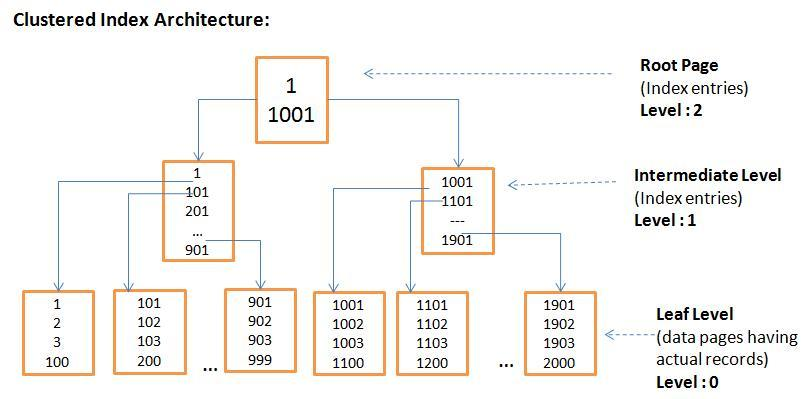
\includegraphics[width=0.9\textwidth]{images/clusteredIndex.jpg}
		\caption{Représentation d'un index \textit{clustered}.\cite{clusteredIndex}}
		\label{clusteredIndex}
	\end{figure}

	Bien évidemment les données peuvent être répliquées en plus d'être éparpillées sur plusieurs machines.


		\section{Les bases de données clé / valeur}
			\subsection{Modélisation}
	Les bases de données clé-valeur sont les bases de données qui possèdent la représentation la plus simple car elles ne contiennent que des paires clé-valeur. Les opérations disponibles sur de telles bases de données sont très limitées :
	\begin{itemize}
		\item Création d'une paire clé-valeur 
		\item Accès à une valeur à partir de la clé
		\item Suppression d'une paire clé-valeur
		\item Incrémentation d'une valeur à partir de la clé
		\item Décrémentation d'une valeur à partir de la clé
	\end{itemize}
	\vspace{20px}
	Quelques autres opérations classiques sur les listes sont disponibles pour certains moteurs : ajout d'un élément à une liste, suppression d'un élément, comptage du nombre d'éléments d'une liste\dots\\

	La figure~\ref{commandesRedis} montre quelques exemples de commandes sous Redis, une base de données clé-valeur.

	\begin{listing}[H]
		\inputminted{text}{code/commandesRedis.txt}
		\caption{Quelques exemples de commandes basiques de Redis}
		\label{commandesRedis}
	\end{listing}

\subsection{Cas d'utilisation}

\subsection{Acteurs principaux}
	La popularité des bases de données est donnée par DB-engines\cite{db_engines_key_value} pour le mois de septembre 2014.

	\begin{enumerate}
		\item \textbf{Redis}. Première version en avril 2009, écrit en C, open-source sous licence BSD. Le développement a été sponsorisé par VMware et Pivotal Software. Utilisé par The Guardian, GitHub, Stack Overflow, YouPorn, Twitter etc.\cite{Wikipedia_redis}
		\item \textbf{Memcached}. Première version en mai 2003. Écrit en C, open-source sous licence BSD. Le développement a été sponsorisé par Danga Interactive. Utilisé par Reddit, Facebook, Orange, Tumblr, Wikipedia etc. Il est connu pour utiliser une gigantesque table de hash, distribuée sur plusieurs machines. Quand la table est pleine, les données sont supprimées à l'aide de la méthode du LRU\footnote{LRU : \textit{Least recently used}.}.\cite{Wikipedia_memcached}
		\item \textbf{Riak}. Première version en août 2009, écrit en Erlang, open-source sous licence Apache 2.0. Le développement est assuré par Basho Technologies, qui propose une offre payante cloud. Utilisé par AT\&T, Boeing, Rovio, Yahoo! etc.\cite{Wikipedia_riak}
	\end{enumerate}


		\section{Les bases de données orientées documents}
		\label{sec:BDDDocuments}

		\section{Les bases de données orientées graphes}

		\section*{Conclusion}
			Cette partie a présenté les implémentations les plus courantes du NoSQL permettant de résoudre la majorité des problèmes. Le tableau suivant présente un récapitulatif des propriétés de chaque base de données et de leur utilité.\\

TODO : tableau


	%% -- Bibliographie
	\bibliographystyle{plain}
	\bibliography{bib}
\end{document}
